\chapter{Introduction}\label{sec:introduction}

The discovery of particles at the electroweak scale, such as the top quark at Fermilab's CDF and D0~\cite{topD0,topCDF} and the Higgs boson at the Large Hadron Collider (LHC) in CERN~\cite{higgscms,higgsatlas}, led to the discovery of all constituents in the Standard Model (SM).
The SM describes the nature of fundamental particles and their interactions with precision.
Despite its success, the SM suffers from a few obstacles:
the evidence of neutrino masses and mixing~\cite{neutrino}, the observations of bullet clusters confirming the presence of dark matter (DM)~\cite{Baumgart:2009tn,Kaplan:2009ag,Chan:2011aa,Dienes:2011ja,Dienes:2012yz}, and baryon-antibaryon asymmetry~\cite{Cui:2014twa} all remain unexplained in the framework of SM.
In addition, the SM suffers from the naturalness problem.
One needs to look for physics Beyond the Standard Model (BSM) to solve such issues.

To search for the BSM, the high energy physics (HEP) community has completed many types of research, both on the theoretical and experimental sides.
The theoretical high energy physics community approached the issue with two main approaches.
The first approach tackles the issue of precision.
Although the SM is a well-constrained model, further precision of particles in the SM, especially those in the electroweak scale, gives new insight into BSM physics.
For instance, the CDF collaboration recently discovered a 7$\sigma$ deviation of the W boson mass from the SM prediction~\cite{Aaltonen:2022aaa}.
The W boson mass deviation has been interpreted for new physics using the framework of the Standard Model Effective Field Theory (SMEFT)~\cite{Mishima:2022aab}.
In SMEFT, the SM operators from the SM Lagrangian are used to build 5,6,8-dimensional new terms for the Lagrangian.
The SMEFT scalar, fermion, or vector extension hints at new insight into the BSM and its phenomenology~\cite{Mishima:2022aab}.
The other approach aims to build an entirely new Lagrangian term, which can be appended to the current SM Lagrangian term.
The BSM Lagrangian introduces new particle fields and should address unsolved issues in the current SM framework.
The new particles' mass scale can range from the collider level to the astrophysical level.






To find the new BSM particles, the experimental high energy physics community conducted many different kinds of research based on collider and astrophysical data.
Experimental physicists invested strenuous effort in data from collider physics since the lightest particles from popular theory, such as supersymmetry (SUSY), were within the collider's hard scattering energy level.
Experimentalists searching for the BSM particles can also divide their main approaches into 2, the first with prompt decay of the BSM particle and the second with a long-lived lifetime signature.
CMS analysis targeting the BSM particles with prompt lifetime has been exhaustively studied and resulted in no deviation from the SM prediction ~\cite{SUSY}.
However, the second approach, which has not been fully investigated, is when particles decay with a Long-Lived signature, in other words, Long-Lived particles (LLP).
This signature is uniquely exciting and challenging for scientists.
It requires a different analysis strategy depending on the BSM particle's mass scale (MS) and lifetime (c$\tau$).
Thus, HEP experimental scientists perceive this frontier as the blue ocean for HEP experimentalists, to the extent that they are planning a new detector to target LLPs solely ~\cite{Barron:2022aac}.

In this dissertation, we focus on the LLPs originating from the LHC, specifically CMS, review precedent analyses, and propose a novel strategy.
Searches for LLPs decaying into final states containing jets were investigated
at the Tevatron ( $\sqrt{s}$ = 1.96~TeV) by both CDF~\cite{Aaltonen:2011rja} and D0~\cite{Abazov:2009ik} Collaborations,
at the LHC by the ATLAS and LHCb Collaborations at $\sqrt{s}$ = 7~TeV~\cite{ATLAS:2012av,Aaij:2014nma},
by CMS, ATLAS and LHCb Collaborations at $\sqrt{s}$ = 8~TeV~\cite{Aad:2015uaa,Aad:2015rba,PhysRevD.91.012007,Aad:2015asa,Aaij:2017mic,Aaij:2016xmb,Aaij:2015ica}.
More recently, by CMS ~\cite{Sirunyan:2017jdo,displacedvertices,displacedjets2016,delayedjets,emergingjets,CMS-PAS-EXO-19-021}
 and ATLAS Collaborations ~\cite{Aaboud:2018iil,Aaboud:2018jbr,Aaboud:2018arf,Aaboud:2018aqj,Aaboud:2018kbe,Aaboud:2019trc,Aaboud:2019opc,Aad:2019kiz,Aad:2019pfm,Aad:2019tcc,Aad:2019xav,Aad:2019tua} at $\sqrt{s}$ = 13~TeV.

CMS Collaboration released a new result in 2021.
In the new paper, the Higgs decaying into LLPs is created in association with a Z vector boson \cite{ZHAN}.
This analysis' Feynman diagram is displayed in figure \ref{fig:ZHfeyn}.
The new analysis sheds light on LLPs with lighter masses thanks to the clean dilepton trigger from the Z vector boson.
The precedent analyses successfully put the exclusion limit on the branching ratio, the Higgs to the LLPs to b and d-quark, below unitarity. 
However, the exclusion limit for $\tau$ final state has been omitted or presented with values above 1.

\begin{figure}[h!]
  \caption{Feynman diagram of ZH signal process studied in the most recent CMS analysis paper (2021) \cite{ZHAN}}
  \label{fig:ZHfeyn}
  \centering
  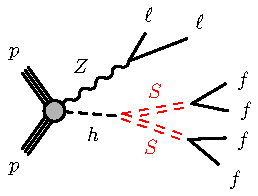
\includegraphics[width=0.47\linewidth]{figs/Zh-llffff-SS.pdf}
\end{figure}


However, the Leptophilic model for Twin Higgs and other Higgs models are also highly motivated ~\cite{Lepto}. Continuous neglect of $\tau$ final state limit is not only poor practice but overlooks an important unexplored phase space.
This analysis searches for LLPs originating from the Higgs Portal model with the Higgs' Leptophilic nature.
Since the coupling strength of the Higgs' to SM fermions are quantified by the Yukawa couplings, focus on Leptophilic Higgs translates into a focus on $\tau$ final state decaying back from the LLPs via the Higgs Portal.
The mass limit on the scalar mass is 55GeV; we investigate only on-shell neutral scalar particles from the Higgs.
A minimum 7 GeV mass for scalar particles is required to create on-shell $\tau$-lepton pairs.
Feynman's scalar particle production mechanism diagram is depicted in Figure \ref{fig:sig}.
%Displaced Jets analyses face challenges for $\tau$ final state due to $\tau$'s non-trivial hadronic and leptonic decay modes and complicated reconstruction mechanism. 
The main challenge and reason for omitting a $\tau$ lepton analysis are the different decay modes of $\tau$ leptons.
$\tau$ leptons decay hadronically and leptonically, with several different sub-decay modes.
Its decay mode pie chart and CMS detection category pie chart are displayed in figures of \ref{fig:tdecay} and \ref{fig:tdet} respectively.
Developing analysis strategies to optimize the search for each sub-decay mode is exceptionally complicated—the main reason for the omission or no reasonable exclusion limit in precedent LHC results.
A displaced vertex search can be more efficient than displaced objects (jet, muon, electrons) search to be inclusive of all $\tau$ leptons' decay modes.
We exploit the newly developed Regions of Interest mechanism in the tracker volume.
Regions of Interest (ROI) form displaced vertex candidates by fitting pair-wise tracks of Lost-tracks and PackedPFCandidates classes in MINIAOD data into a vertex.
ROIs save all relevant track and fitted vertex qualities along with isolation information.
These variables are input for Machine Learning (ML) algorithms, enabling a highly generic and data-scientific search method.

\begin{figure}[h!]
  \caption{The analysis' signal process feynman diagram. The Higgs is created in gg production mode. The LLP scalar decays into $\tau$ lepton.}
  \label{fig:sig}
  \centering
  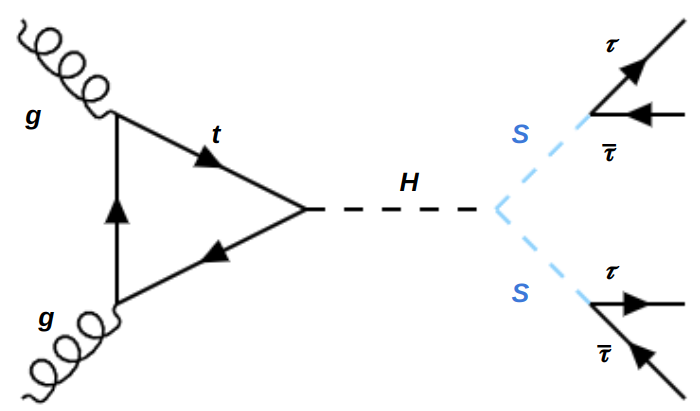
\includegraphics[width=0.47\linewidth]{figs/sigprocess.png}
\end{figure}


\begin{figure}[h!]
  \caption{$\tau$ lepton's decay mode pie chart}
  \label{fig:tdecay}
  \centering
  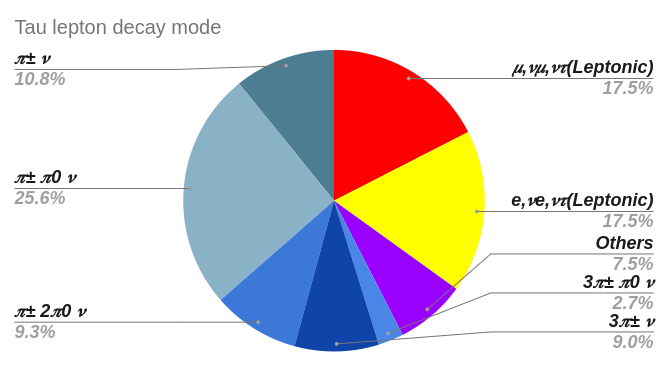
\includegraphics[width=0.87\linewidth]{figs/Taudec.png}
\end{figure}

\begin{figure}[h!]
	\caption{$\tau$ lepton's detection mode pie chart. Prong means a charged track reconstructed in the tracker volume of CMS. It corresponds to $\pi^{\pm}$}
  \label{fig:tdet}
  \centering
  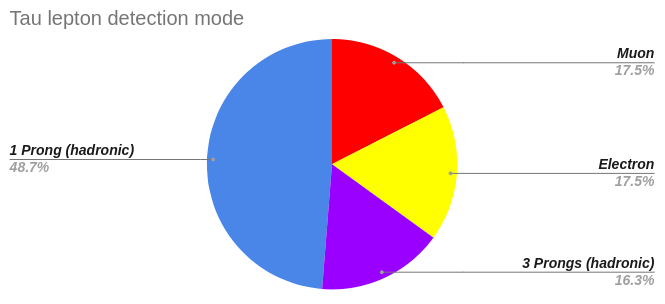
\includegraphics[width=0.87\linewidth]{figs/Taudet.png}
\end{figure}


Another challenge is that CMS searches are not optimal for detecting Higgs boson decays due to its decay products' soft $p_T$ nature.
Higgs produced in association with Z vector boson analysis~\cite{ZHAN} overcame this barrier with the help of dilepton trigger.
Although the ggH production mode gives the most significant Higgs cross-section, it further complicates the trigger strategy.
This analysis exploits the $\tau$ lepton's leptonic decay, where the $\tau$ lepton decays into a soft muon.
We use a trigger of the B Parking High-Level Trigger (HLT) Path implemented in CMS for the 2018 portion of Run 2 to trigger on the soft muon.



The rest of the dissertation is organized as follows.
In Section~\ref{sec:theory}, we discuss the theoretical background of the BSM and LLPs in more detail.
In Section~\ref{sec:detectors}, CMS detector is thoroughly discussed with emphasis on the tracks and the calorimeter, which are relevant detector parts for the analysis.
We discuss how the analysis exploited the b-parking trigger in Section~\ref{sec:triggers}, with a description of its original motive for the trigger's installation.
The physics objects and formation of Regions of Interest are clarified in Section~\ref{sec:objects}.
The machine learning algorithms are further explained in Section~\ref{sec:machinelearning}.
The event selections are presented in Section~\ref{sec:selections}.
Section~\ref{sec:estimate} describes the data driven background estimation method.
Section~\ref{sec:systs} describes the background estimation method's validation process and systematic uncertainties.
Finally, Section~\ref{sec:results} presents the search results.
We conclude with Section~\ref{sec:conclusions}.




%Standard CMS searches rely on $H_T$ triggers that are highly inefficienty for this signal.
%Low hadronic activity in transverse signature becomes particularly more difficult with a long-lived signature.
